\section{Методы обнаружения сигналов}
\label{sec:theory}


\subsection{Общие сведения}

Обнаружение сигналов является фундаментальной задачей радиосвязи. Потребность в этом возникает в большинстве сценариев использования радиосредств, причем, каждая сфера применения определяет эту проблему по-своему. Пользовательским радиоприемникам нужно сканировать заданный диапазон на наличие наиболее мощных сигналов, которые достаточно сильно выделяются на общем фоне и непрерывны во времени. В служебной связи задача осложняется тем, что зачастую канал можно обнаружить только во время его использования. При дальней связи и связи в неблагоприятных условиях полоса частот известна заранее, но мощность сигнала меньше мощности шума, тогда обнаружить его означает подобрать подходящую модель, чтобы компенсировать помехи и извлечь полезную информацию. В сфере радиоразведки ведется постоянная гонка вооружений и данная проблема актуальна всегда.

Такое многообразие задач, имеющих общее название "<обнаружение сигналов">, очевидно, не может быть охвачено небольшим набором методов. Тем не менее, в их решении есть общая основа  --- представление сигнала. Радиоволна имеет вполне определенные физические характеристики, которые исследователь может представить в любой удобной для него форме.
Наиболее интуитивное их выражение --- это последовательность мгновенных уровней сигнала во времени. Оно полезно тем, что существует много методов для работы с временными рядами. Таким образом можно использовать достижения других областей науки и привносить в них свои новшества. Такой подход называется представлением сигнала во временном домене.
В этой форме, однако, не очевидно, как энергия волн распределена по частотам. А это свойство очень полезно, так как нас интересует, на каких частотах наблюдается активность. Поэтому, широкое применение нашел альтернативный подход --- представление сигнала в частотном домене. Оно не привносит новой информации, а является альтернативной формой записи параметров радиоволн. Переход от одного представления к другому осуществляется через прямое и обратное преобразование Фурье, о котором более подробно будет рассказано ниже.

Эти представления лежат в основе двух семейств методов: анализа временных рядов и спектрального анализа. Они решают разные задачи и дополняют друг друга.


\subsection{Авторегрессионная модель}

Авторегрессионная модель --- это математическая модель случайного процесса, основывающаяся на предположении, что последующее значение последовательности линейно зависит от предыдущих (\autoref{eq:theory:ar}).

\begin{equation}
  \label{eq:theory:ar}
  X_t = c + \sum_{i=1}^p \phi_i X_{t-i} + \varepsilon_t
\end{equation}
\begin{explanation}
\item[где] $c$ --- константа,
\item $\phi_1, \dotsc, \phi_p$ --- параметры модели,
\item $\varepsilon_t$ --- шум.
\end{explanation}

Это достаточно простая конструкция, которая, впрочем, демонстрирует неплохие результаты и применяется как составная часть более сложных моделей.
Ее основные достоинства --- невысокая вычислительная сложность и возможность применения к любому временному ряду без его анализа. Так можно получать базовое качество оценки параметров ряда и использовать его для получения предварительных выводов.
Недостатки вытекают из простоты --- неспособность уловить сложные закономерности и неустойчивость к шуму.


Настройка авторегрессии заключается в подборе ее параметров. Это делается с помощью метода наименьших квадратов. Количество параметров называется порядком модели и записывается АР(n). Порядок подбирается вручную или методами выбора модели (AIC, BIC и другими). Он не должен быть слишком большим --- в этом случае невязка с данными, используемыми для настройки будет мала, а на новых сильно возрастет. Эта проблема известна как переобучение, то есть излишняя подстройка под обучающие данные, в результате чего страдает обобщающая способность модели.

Теоретически АР обоснована только для случайных процессов, обладающих свойством слабой стационарности, то есть математическое ожидание не изменяется во времени и функция автоковариации постоянна для сдвига $k$:

\begin{equation}
  \begin{split}
    E[X_t] & = const \\
    cov(X_{t_1}, X_{t_1-k}) & = cov(X_{t_2}, X_{t_2-k})
  \end{split}
\end{equation}

Это утверждение неверно применительно к радиосигналам, поэтому авторегрессионная модель в реальных ситуациях обладает слабой предсказательной силой, но по ее поведению все-равно можно сделать некоторые выводы о природе случайного процесса. Например, наблюдая за значениями невязки модельных и реальных данных можно заметить разладки в СП --- невязка резко возрастет.

Тем не менее, на очищенных от шума данных авторегрессия работает неплохо. АР(2) достаточно хорошо приближает модельный FM сигнал (\autoref{fig:theory:ar_pred_next}). Визуально отличия заметны только при детальном рассмотрении. Это можно объяснить гладкой формой синусоиды: каждое следующее значение не сильно отклоняется от предыдущих. При добавлении шума результат становится значительно хуже.

\begin{figure}[h]
  \centering
  \begin{subfigure}{0.45\textwidth}
    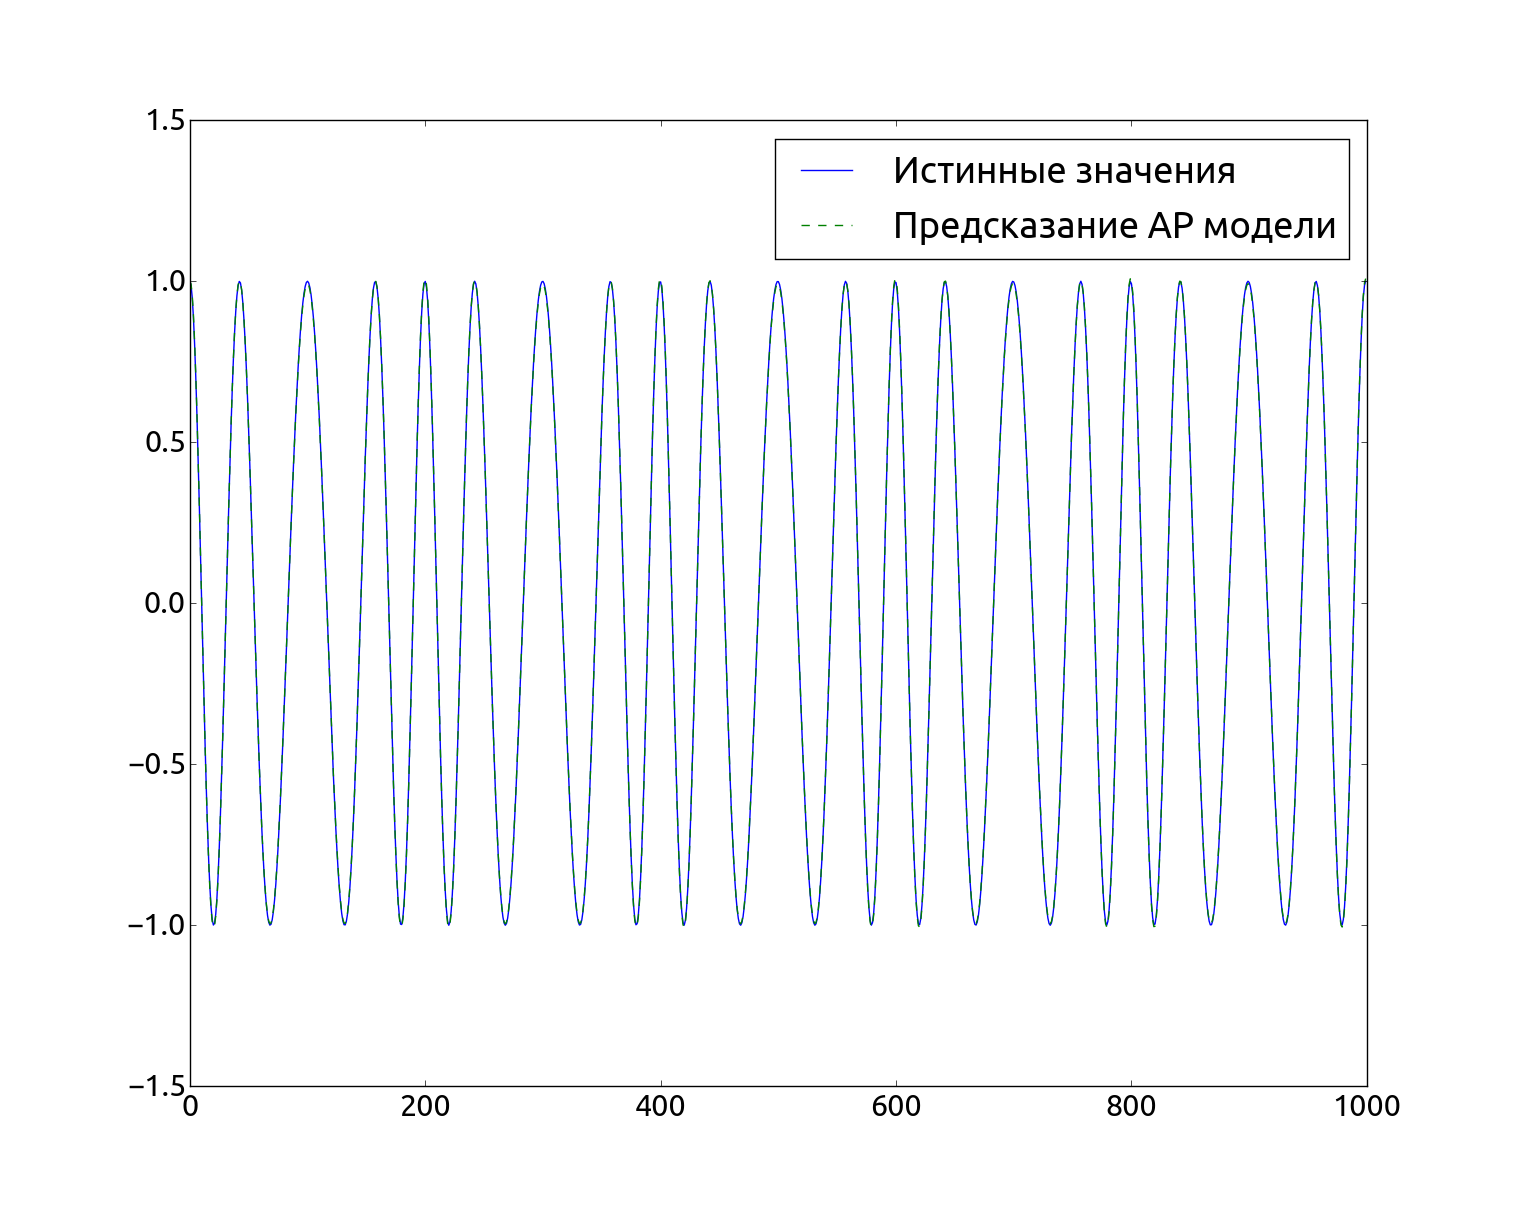
\includegraphics[width=\textwidth]{theory/ar_pred_next}
    \caption{}
    \label{fig:theory:ar_pred_next_whole}
  \end{subfigure}
  \begin{subfigure}{0.45\textwidth}
    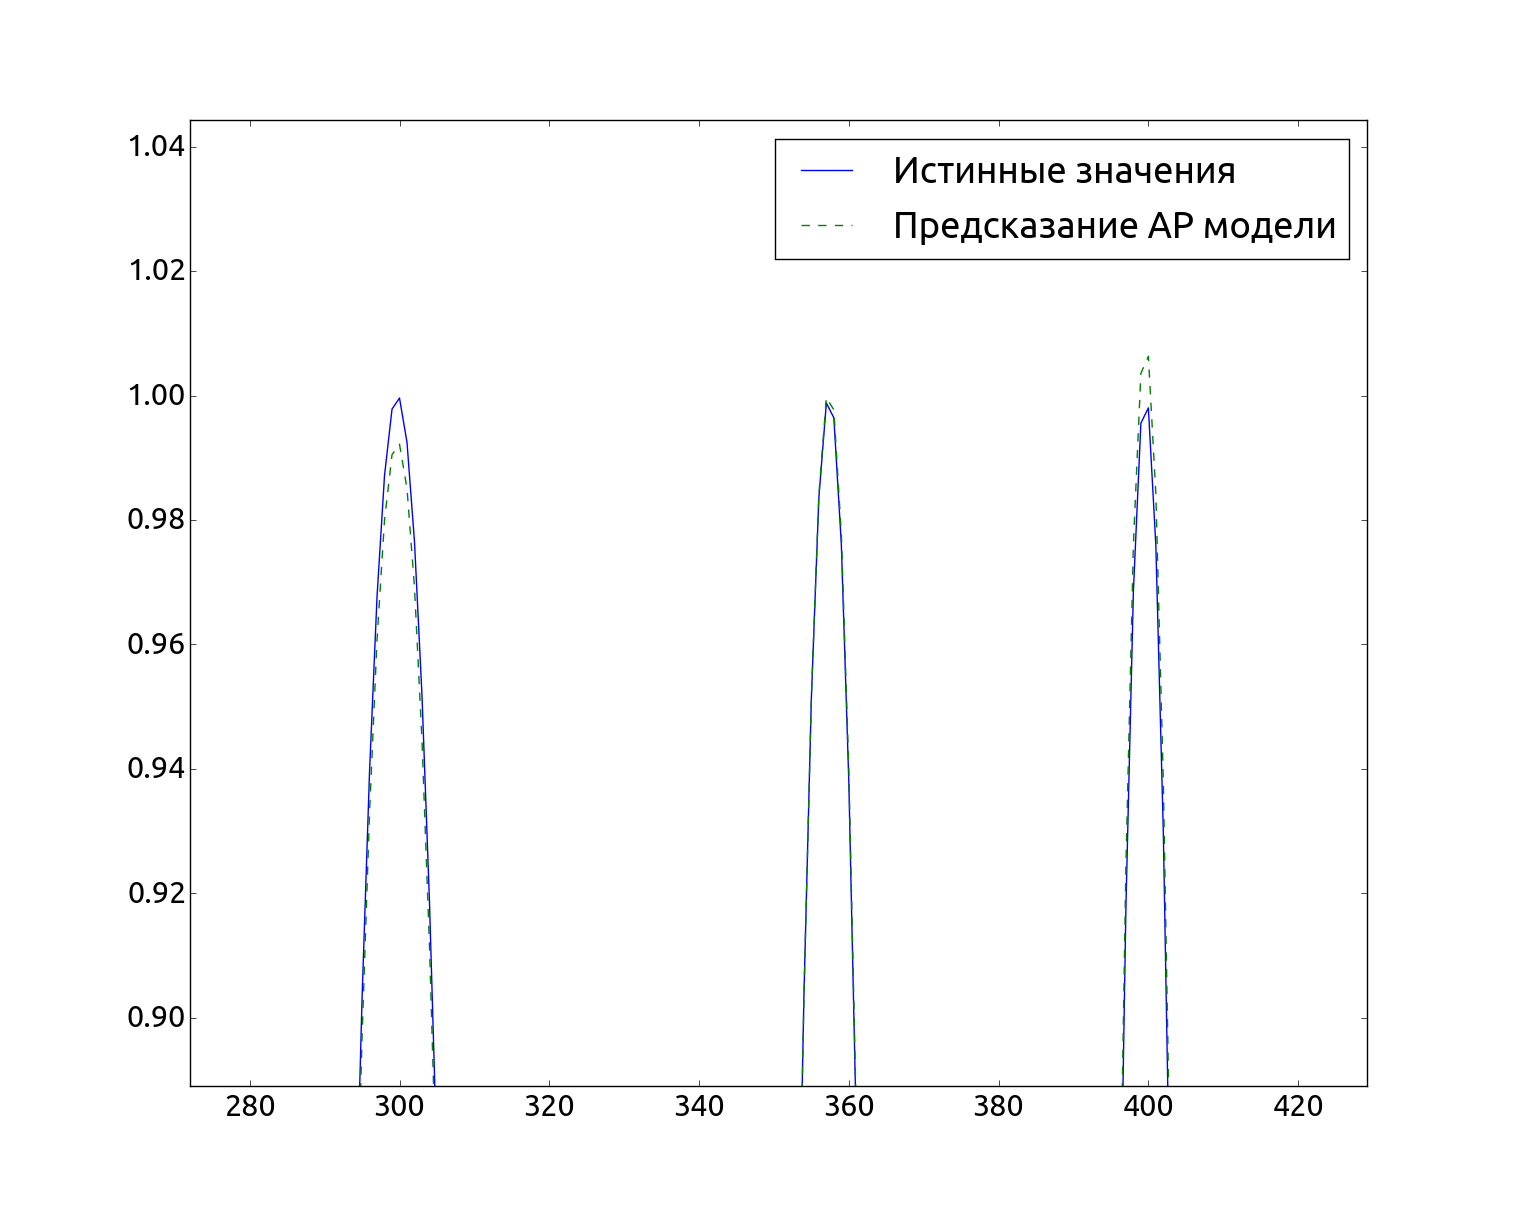
\includegraphics[width=\textwidth]{theory/ar_pred_next_zoomed}
    \caption{}
    \label{fig:theory:ar_pred_next_zoomed}
  \end{subfigure}
  \caption{Предсказания АР модели на основе реальных данных (\subref{fig:theory:ar_pred_next_whole}). Увеличенный участок графика (\subref{fig:theory:ar_pred_next_zoomed}).}
  \label{fig:theory:ar_pred_next}
\end{figure}

Чтобы построить этот график, были сгенерированы два временных ряда. Оба представляют собой частотно модулированную синусоиду. На первом была настроена АР(2), а второй использовался для контроля качества. Из него выбирались два последовательных элемента, и модель на их основе предсказывала следующий. Так был составлен ряд предсказаний модели. Как видно, она достаточно хорошо подстроилась под параметры сигнала. Ошибки можно заметить, если увеличить области перегибов синусоиды: сложно угадать точный угол при изменяющейся частоте.

Интересный эффект можно получить, если строить регрессию на ранее предсказанных данных. Ошибка модели накапливается и усиливается со временем, из-за чего сигнал обычно либо угасает, либо устремляется в бесконечность. Поэтому в расчетах стоит использовать только несколько ближайших предсказанных значений. Зато, при появлении новых наблюдений реальных значений не требуется перестраивать модель, ее параметры действительны, если описываемый случайный процесс не изменил своих параметров.

\begin{figure}[h]
  \centering
  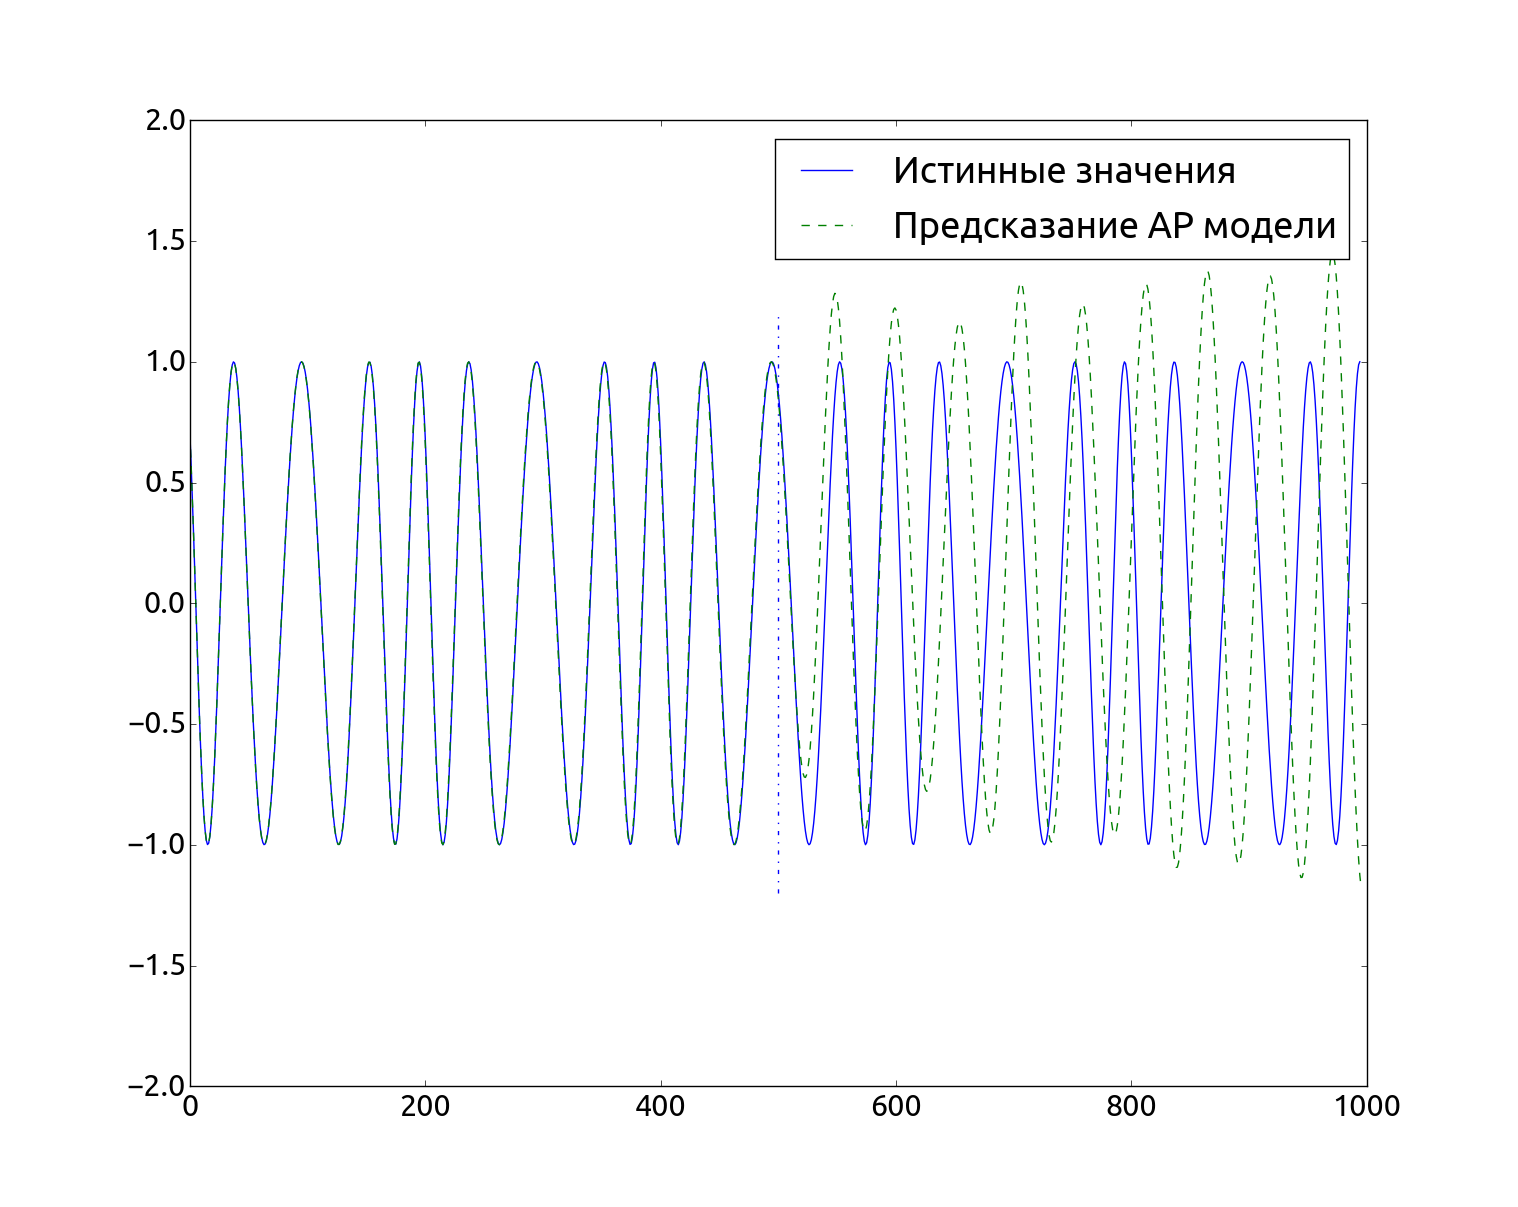
\includegraphics[width=0.9\textwidth]{theory/ar_pred_all}
  \caption{Предсказания АР модели на основе ранее предсказанных ей значений. Вертикальная линия отмечает начало модельных данных.}
  \label{fig:theory:ar_pred_all}
\end{figure}
